\chapter{Pendahuluan}
Bahasa pemrograman Python mulai populer saat dikarenakan berbagai hal; mudah
dipelajari, tersedia dan banyak {\em library}-nya. Nanti akan kita bahas beberapa
library Python ini. Lengkapnya library ini juga yang menyebabkan
Python dipergunakan di berbagai aplikasi. Berbagai sekolah (dan
perguruan tinggi) bahkan mengajarkan Python sebagai pengantar pemrograman.

Bahasa Python dianggap agak ``mudah'' digunakan sehingga dapat diajarkan
kepada orang-orang yang tidak memiliki latar belakang pendidikan pemrograman.
Jadi Python digunakan oleh orang-orang di bidang Biologi sampai Bahasa.
Manager-manager yang ingin belajar statistik atau {\em data science}
dapat menggunakan bahasa Python ini.
Alternatifnya adalah belajar menggunakan bahasa R, tetapi kalau 
nanti ingin melakukan pemrograman untuk yang lainnya lagi harus belajar
bahasa pemrograman lagi. Daripada seperti itu, lebih baik belajar satu
bahasa saja. Pilihannya adalah bahasa Python.

Bahasa Python merupakan sebuah {\em interpreted language} berbeda dengan
bahasa C yang {\em compiled}. Pada bahasa yang {\em compiled}, kita memiliki
kode sumber ({\em source code}) yang harus dirakit ({\em compile}) dahulu
sampai menjadi kode mesin yang langsung dapat dieksekusi pada komputer
yang bersangkutan. Ketika algoritma salah, maka kode sumber harus diperbaiki
dahulu kemudian di-{\em compile}) sebelum dapat dijalankan. Prosesnya
menjadi agak panjang. Sementara itu untuk bahasa yang {\em interpreted},
program langsung dieksekusi dari kode sumbernya (tanpa perlu proses kompilasi).
Dahulu program yang {\em compiled} lebih cepat dalam eksekusinya karena
tidak perlu menerjemahkan baris perbaris ketika dijalankan, namun sekarang
perbedaannya sudah tipis.

Bahasa Python tersedia untuk berbagai sistem operasi; Windows, Mac OS, dan
berbagai variasi dari UNIX (Linux, *BSD, dan seterusnya). Di dalam buku ini
saya akan menggunakan contoh-contoh yang saya gunakan di komputer saya yang
berbasis Linux Mint. Meskipun seharusnya semuanya kompatibel dengan berbagai
sistem operasi, kemungkinan ada hal-hal yang agak berbeda. Jika hal itu
terjadi, gunakan internet untuk mencari jawabannya.

\section{Instalasi}
Python dapat diperoleh secara gratis dari berbagai sumber. Sumber utamanya
adalah di situs python.org. Untuk sementara ini bagian ini saya serahkan kepada
Anda. Ada terlalu banyak perubahan sehingga bagian ini akan cepat kadaluwarsa.
Untuk sistem berbasis sistem operasi Microsoft Windows, biasanya instalasi 
Python menggungankan {\em Anaconda}. (Informasi mengenai ini juga dapat
dilihat pada situs python.org.)

Untuk sistem operasi berbasis Linux dan Mac OS, Python sudah terpasang sebagai
bawaan dari sistem operasinya. Jika Anda ingin memasang versi terbaru maka
Anda harus memasangnya sendiri dengan mengunduh instalasinya di python.org.
Atau, jika Python sudah terpasang di komputer Anda, maka Anda dapat melakukan
{\em upgrade}.

\section{Python Tanpa Instalasi - Google Colab}

Ada cara lain menggunakan Python adalah dengan menggunakan layanan
{\bf Google Colabs}, yang mana kita diberikan akses ke sebuah mesin virtual
yang sudah terpasang Python. Python berada di {\em cloud}.
Untuk pendekatan ini kita tidak perlu memasang Python lagi. 
Lebih mudah untuk belajar dan bahkan untuk membuat prototipe.

Bagi saya, sebagai seorang dosen, pemanfaatan Google Colab ini
sangat menarik karena siswa akan memiliki konfigurasi yang sama.
Seringkali kalau mengajar di kelas dengan komputer yang berbeda-beda 
(beda sistem operasi, beda versi Python, letak instalasi, beda versi
dari {\em library}, dan seterusnya), waktu dan tenaga akan habis untuk 
mengurusi hal-hal yang tidak jalan karena perbedaan tersebut.
Bagi Anda yang mengajar Python, saya sarankan untuk menggunakan
pendekatan dengan menggunakan Google Colab ini.

Buku ini akan diperbaharui dengan cara menggunakan Google Colabs ini.

\begin{figure}
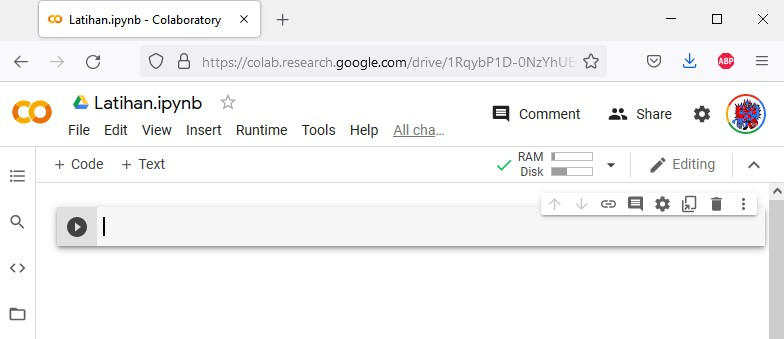
\includegraphics[width=1.0\linewidth]{graphics/google-colab.jpg}
\caption{Tampilan Google Colab}
\end{figure}

Layanan Google Colab dapat diakses dengan menggunakan {\em browser} dan
diarahkan ke alamat colab.research.google.com (atau gunakan search engine
untuk mencapai domain tersebu).
Setelah ditampilkan halaman depan, kita dapat membuka program baru dengan
membuka {\em New Notebook} atau membukan kodingan lama kita yang sudah
disimpan di akun Google Drive kita.
Google colab menyediakan sebuah komputer virtual yang dapat kita gunakan
untuk melakukan pemrograman dalam bahasa Python (yang dalam hal ini dapat
kita pilih mau menggunakan versi 2 atau 3).

\section{Memulai}
Untuk memastikan Python berjalan, ketikkan ``python'' di terminal Linux Anda.
(Bagi yang menggunakan Windows, hal ini dapat dilakukan dengan menggunakan
CMD.exe.) Catatan, di sistem Linux, tanda ``dollar'' (atau persen)
merupakan {\em prompt} dari {\em shell} Anda. Jangan diketikkan.
Di beberapa sistem yang memiliki instalasi Python~2 dan Pyhton~3 secara
bersamaan, ada kemungkinan Anda harus mengetikkan ``python3''
(perhatikan ada angka ``3'').
Di kemudian hari, {\em default} dari perintah `python' akan mengacu
kepada versi 3.

\begin{verbatim}
$ python
Python 2.7.12 (default, Nov 20 2017, 18:23:56) 
[GCC 5.4.0 20160609] on linux2
Type "help", "copyright", "credits" or "license" for more information.
>>> 
\end{verbatim}

Dari tampilan di atas dapat kita ketahui bahwa Python yang saya gunakan adalah
versi 2.7.12\footnote{Pada awal penulisan buku ini, versi bahasa Python Yang
stabil digunakan adalah versi 2. Saat ini versi~3 merupakan versi yang dianggap
sebagai versi stabil. Untuk itu buku ini sedikit demi sedikit akan diperbaharui
dengan menggunakan Python versi 3.}. 

\begin{verbatim}
% python3
Python 3.9.10 (main, Jan 15 2022, 11:40:53) 
[Clang 13.0.0 (clang-1300.0.29.3)] on darwin
Type "help", "copyright", "credits" or "license" for more information.
>>> 
\end{verbatim}

Sekarang kita dapat memulai pemrograman Python dengan menuliskan
program ``hello world'' (yang merupakan standar bagi belajar pemrograman).
Ketikkan ``print ...'' (dan seterusnya seperti di bawah ini).

\begin{verbatim}
print("Hello, world!")
Hello, world!
\end{verbatim}

Python akan menampilkan apapun yang ada di antara tanda petik tersebut. Hore!
Selamat! Anda berhasil membuat program Python yang pertama.

Ada beberapa cara untuk menjalankan Python. Pada contoh di atas, kita
menjalankannya secara langsung. Cara ini memang yang paling cepat, tetapi ada
banyak hal yang harus kita lakukan secara manual. Sebagai contoh, jika kita
ingin membuat sebuah {\em block}, maka kita harus mengetikkan sendiri empat
spasi untuk membuatnya masuk. Jika ini tidak kita lakukan, maka dia akan
``marah'' dan menampilkan pesan. Berikut ini contoh sesi yang salah.

\begin{verbatim}
$ python3
Python 3.5.2 (default, Nov 23 2017, 16:37:01) 
[GCC 5.4.0 20160609] on linux
Type "help", "copyright", "credits" or "license" for more information.
>>> for i in range(10):
... print(i)
  File "<stdin>", line 2
    print(i)
        ^
IndentationError: expected an indented block
>>> 
\end{verbatim}

Pada contoh di atas, kesalahan terjadi karena kita tidak memberikan spasi di
depan perintah ``print(i)''. Seharusnya kita melakukan hal seperti ini.
(Perhatikan spasi sebelum kata ``print''.)

\begin{verbatim}
$ python3
Python 3.5.2 (default, Nov 23 2017, 16:37:01) 
[GCC 5.4.0 20160609] on linux
Type "help", "copyright", "credits" or "license" for more information.
>>> for i in range(10):
...     print(i)
... 
0
1
2
3
4
5
6
7
8
9
>>> 
\end{verbatim}


Mari kita lanjutkan dengan membuat program yang lebih panjang. Program Python
dapat disimpan di dalam sebuah berkas untuk kemudian dieksekusi belakangan.
Buka editor kesukaan Anda dan ketikkan program hello world di atas di dalam
editor Anda tersebut. Setelah itu simpan berkas tersebut dengan nama
``hello.py''. Biasanya berkas program Python ditandai dengan akhiran
(extension) ``.py''.

Setelah berkas tersebut tersedia, maka kita dapat menjalankan Python dengan
memberikan perintah python dan nama berkas tersebut. 
Kata ``Hello world'' akan ditampilkan.

\begin{verbatim}
$ python hello.py
Hello, world!
\end{verbatim}

Cara lain yang dapat dilakukan adalah dengan menggunakan program IPython,
yaitu interactive Python. Biasanya program IPython ini belum terpasang di
sistem operasi bawaan komputer Anda. Tinggal unduh dari ipython.org.
(Perhatikan IPython ini sudah mengenal {\em syntax} dari Python sehingga 
ketika kita mengetikkan {\em for loop} maka dia akan memberikan spasi 4 buah
sebagai {\em indentation}.)

\begin{verbatim}
$ ipython3
In [1]: print("Hello World")
Hello World

In [2]: for i in range(10):
   ...:     print(i)
   ...:     
0
1
2
3
4
5
6
7
8
9

In [3]: 
\end{verbatim}

Masih ada satu cara lain menjalankan program Python, yaitu dengan menggunakan
Jupyter. Yang ini akan kita bahas secara lebih khusus.

Pada contoh-contoh di atas hasil print dicetak ke bawah. Bagaimana jika kita
ingin hasil cetaknya tidak turun ke bawah atau tanpa {\em newline}?
Cara berikut ini - dengan menambahkan (end = " ") - dapat digunakan:

\begin{verbatim}
for n in range(10):
   print(n, end=" ")
\end{verbatim}
Keluaran dari program di atas adalah cetakan yang ke kanan.
\begin{verbatim}
0 1 2 3 4 5 6 7 8 9
\end{verbatim}


\section{Shell atau IDE}
Pemrograman Python dapat dilakukan dengan editor seperti yang sudah ditunjukkan
di atas dan kemudian menjalankannya secara {\em command line} di shell,
Cara lain yang lebih sering dilakukan orang adalah menggunakan sebuah
Integrated Development Editor (IDE) untuk melakukan pemrogramannnya.
Menjalankan kodenya dapat dikomandokan dari IDE atau dari shell juga.

Ada beberapa IDE untuk Python, seperti misalnya IDLE.
Yang sekarang sedang naik daun adalah dengan menggunakan {\em Jupyter Notebook}.
Yang menarik dengan pendekatan ini adalah kita melakukan dokumentasi dan
pemrograman sekaligus di lingkungan tersebut.
Google Colab pun sesungguhnya menggunakan konsep Jupyter Notebook ini tetapi
membawanya ke lingkungan {\em cloud}.
Nanti ini akan kita bahas dengan lebih lanjut.

\section{Bahasa Python} 
Tentang bahasa Python itu sendiri akan diperdalam pada versi berikutnya.
Sementara itu fitur tentang bahasa Python akan dibahas sambil berjalan.
Pendekatan ini saya ambil untuk membuat buku menjadi lebih menarik dan lebih
singkat. Belajar seperlunya. Mari kita mulai.

Variabel di dalam Python langsung dapat digunakan tanpa melakukan deklarasi
sebelumnya. Pada bahasa pemrograman seperti C, variabel harus dideklarasikan
tipenya; apakah dia {\em integer} atau {\em string}.
Contohnya di bawah ini.
\begin{verbatim}
a = 7
b = 5
print(a,b)
\end{verbatim}
Pada contoh di atas, variabel $a$ dan $b$ dibuat dan langsung diisi dengan
angka (7 dan 5) dalam kasus ini.
Kemudian kedua variabel tersebut disampaikan sekaligus.
Perhatikan bahwa dengan menggunakan tanda koma (,) nilai dari kedua variabel
tersebut ditampilkan dengan spasi.

\begin{verbatim}
7 5
\end{verbatim}

Berikut ini kita buat penampilan yang lebih ``menarik'' (untuk Python3).
\begin{verbatim}
a = 7
b = 5
c = a + b
print ("a = ", a)
print ("b = ", b)
print ("a+b = ", c)
\end{verbatim}

Keluaran dari Python3 adalah seperti ini:
\begin{verbatim}
a = 7
b = 5
a+b = 12
\end{verbatim}

Hal yang sangat berbeda dari bahasa Python dengan
bahasa pemrograman lainnya adalah masalah {\em block} dari kode. 
Bahasa pemrograman C misalnya menggunakan tanda kurung kurawal ``\{'' 
untuk menyatakan blok. Sementara itu Python menggunakan {\em indentation} 
untuk menyatakan satu blok. Lihat contoh di bawah ini.

\begin{verbatim}
for i in range(5):
    for j in range(3):
        print(i,j)
\end{verbatim}

Disarankan untuk menggunakan spasi sebanyak empat (4) buah untuk {\em
indentation} tersebut. (Ini membuat banyak perdebatan karena ada banyak orang
yang menggunakan tab bukan spasi.)

Mari kita buat contoh-contoh lain. Apa keluaran program di bawah ini?
\begin{verbatim}
nama1 = "budi"
nama2 = "rahardjo"
nama3 = nama1 + nama2
print(nama3)
\end{verbatim}

Perhatikan bahwa untuk variabel yang berjenis angka (integer) maka operator 
tambah (+) akan menambahkan angkanya. Sementara itu pada variabel yang
berjenis {\em string}, operator (+) akan menyambungkan ({\em concatenate})
variabel {\em string} tersebut.
Ini merupakan ciri dari sebuah bahasa yang berorientasi obyek
({\em object oriented}).
Untuk tipe data yang lainnya, operator tambah (+) kemungkinan juga akan
memiliki perilaku yang berbeda.

Mari kembali ke data yang berbentuk angka. Apa keluaran dari program
di bawah ini?
\begin{verbatim}
a = 7
b = 5
c = a/b
print(c)
\end{verbatim}

Keluarannya adalah nilai ``1.4''. Jenis atau tipe data dari ``a'' dan ``c''
adalah berbeda. Tipe data ``a'' adalah {\em integer}, sementara itu
tipe data ``c'' adalah {\em floating point}.

\begin{verbatim}
>>> a=7
>>> type(a)
<class 'int'>
>>> b=5
>>> c=a/b
>>> type(c)
<class 'float'>
\end{verbatim}

Bolehkah kita mencampurkan tipe data yang berbeda?
Mari kita lanjutkan dengan contoh di atas.
\begin{verbatim}
d = a+c
print(d)
\end{verbatim}
Keluaran dari kode di atas adalah ``8.4''. Artinya pencampuran tipe data
yang berbeda (dalam hal ini adalah {\em integer} dan {\em float}) dapat
dilakukan. Hasilnya adalah bilangan {\em float}.
Hal ini menunjukkan bahwa bahasa Python dapat dibuat tidak {\em strict}.
Bahasa pemrograman lain - misalnya Java (dan umumnya bahasa pemrograman
yang berorientasi obyek) - sangat ketat dalam hal ini.


\section{Kompleksitas}
Pada bagian sebelumnya kebetulan sempat disinggung tentang {\em loop},
maka pada bagian ini pembahasannya sedikit melebar ke aspek Kompleksitas
(dari subuah algoritme).
Ini memang lebih berbau aspek teoritis dari ilmu komputer.

Ketika seseorang mengembangkan atau menggunakan sebuah algoritme untuk
mengimplementasikan programnya, maka ada satu hal yang perlu diperhatikan
yaitu kompleksitas.
Singkatnya, kompleksitas itu menunjukkan seberapa besar sumber daya yang
akan digunakan (dibutuhkan) untuk menjalankan algoritme tersebut sebagai
sebuah fungsi dari jumlah data yang diproses.
Sebagai contoh, sebuah aplikasi mungkin berjalan dengan baik ketika jumlah
datanya hanya 100, tetapi kemudian menjadi sangat lambat atau bahkan tidak
jalan ketika jumlah datanya 1000 atau lebih.
Nah jumlah data tersebut (100 atau 1000) merupakan sebuah paramter yang
menjadi fungsi dari sumber daya yang digunakan. Biasanya ini kita sebut $n$.
Kompleksitas kemudian menjukkan seberapa besar sumber daya sebagai fungsi
dari $n$ itu.

Ada algoritme yang lama komputasinya bergantung liner terhadap jumlah data
($n$) itu. Jadi misalnya untuk 100 data dibutuhkan 100 detik, maka untuk
1000 data dibutuhkan waktu 1000 detik. Bagaimana jika jumlah datanya 10000?
Maka dapat diperkirakan waktu yang dibutuhkan adalah 10000 detik.
Kompleksitas yang sepert ini disebuh $O(n)$.

Ada juga algoritme yang lama perhitungannya berbanding kuadratis (pangkat dua)
terhadap jumlah datanya. 
Kompleksitas yang model seperti ini disebut $O(n^{2})$


\begin{verbatim}
n=1000
import time

start_time = time.time()
a = 0
for x in range(n):
    a = a + 0
end_time = time.time()
elapsed = end_time - start_time
print("elapsed %s seconds ..." % elapsed)
\end{verbatim}

Contoh kode di atas menunjukkan sebuah {\em loop} dengan 1000 kali putaran.
Jumlah loop ditentukan oleh variabel $n$, yang pada contoh di atas diisi 1000.
Di dalam setiap loop ada perintah {\em dummy}, yaitu variabel $a$ ditambah
dengan bilangan nol. Ini hanya sekedar untuk menunjukkan beban komputasi penjumlahan.
Tentu saja di dalam dunia nyata, komputasiny lebih berat.

Jika program tersebut dijalankan maka dia akan menghasilkan waktu eksekusi
sebanyak $4,5538 \times 10^{-5}$ detik.
Angka tepatnya tentu saja bergantung kepada komputer yang digunakan.
Ini hanya sebagai contoh saja, yang kebetulan diambil dari laptop saya.

Sekarang mari kita tambahkan loop di dalamnya sehingga kodenya menjadi seperti berikut.

\begin{verbatim}
n=1000
import time

start_time = time.time()
a = 0
for x in range(n):
    for y in range(n):
        a = a + 0
end_time = time.time()
elapsed = end_time - start_time
print("elapsed %s seconds ..." % elapsed)
\end{verbatim}

Pada prinsipnya, kita menambahkan sebuah loop lagi di dalam loop sebelumnya.
Jadi di dalam loop yang $x$, kita menambahkan loop $y$ yang jumlah loop-nya
juga sama ($n$). Jika kode ini dijalankan maka dihasilkan keluaran waktu
$0,05148$ detik, atau $5,418 \times 10^{-2}$.
Perhatikan bahwa waktu yang dibutuhkan untuk mengeksekusi ini 1000 kali
lebih besar (lebih lambat) dari waktu sebelumnya.
Kompleksitas dari algoritme ini menjadi $O(n^2)$.

Mari kita tambahkan satu loop lagi di dalam loop $y$ sehingga kodenya menjadi
seperti berikut.

\begin{verbatim}
n=1000
import time

start_time = time.time()
a = 0
for x in range(n):
    for y in range(n):
       for z in range(n): 
           a = a + 0
end_time = time.time()
elapsed = end_time - start_time
print("elapsed %s seconds ..." % elapsed)
\end{verbatim}

Seperti sebelumnya, kode ini kita jalankan juga. Hasilnya adalah $51,1767$ detik.
Atau $5,11767 \times 10$. Perhatikan bahwa ini 1000 kali lebih lambat dari sebelumnya
dan 1 juta kali lebih lambat dari loop yang pertama kali (yang hanya ada $x$).
Kompleksitas dari algoritme ini adalah $O(n^3)$.

Anda boleh mencoba menggantikan angka variabel $n$ tadi dengan 10000.
Namun perlu diingat bahwa waktu yang dibutuhkan untuk menjalankan kode
tersebut menjadi sangat lama. Jika Anda tertarik, coba jalankan.
Berapa detik waktu yang dibutuhkan untuk menjalankan itu?

Apa yang kita bahas ini adalah kompleksitas yang dikaitkan dengan lamanya
(waktu) eksekusi. Ada juga kompleksitas yang terkait dengan besarnya
memori yang dibutuhkan (untuk memproses data).
Ini merupakan bahasan yang lebih kompleks, tetapi prinsipnya sama.

\section{List}
Python memiliki struktur data {\em list}, yang sama dengan {\em array}
(larik) di bahasa pemrograman lainnya. Untuk membuat {\em list} kita
menggunakan tanda siku kotak. Contoh berikut ini menunjukkan penggunaan 
struktur data {\em list}.

\begin{verbatim}
# contoh list di Python
daftar = [7, 1, 5, 3, 2, 4, 6, 8, 3, 5]
print(daftar)
print("list memiliki", len(daftar), "elemen")

# akses elemen yang pertama (dengan indeks 0)
print("daftar[0] =", daftar[0])

# akses ke elemen terakhir
print("terakhir =", daftar[-1])

# menambahkan data ke list
daftar = daftar + [7, 9]
print(daftar)
\end{verbatim}

Keluaran dari kode di atas adalah sebagai berikut.
Perhatikan baris terakhir adalah karena penambahan dua elemen baru
di list.
\begin{verbatim}
[7, 1, 5, 3, 2, 4, 6, 8, 3, 5]
list memiliki 10 elemen
daftar[0] = 7
[7, 1, 5, 3, 2, 4, 6, 8, 3, 5, 7, 9]
\end{verbatim}

Ada banyak hal yang dapat kita lakukan dengan menggunakan struktur data
{\em list} ini. Kita dapat menghapus ({\em delete},{\em remove}) 
elemen di daftar tersebut.
Kita juga dapat memotong ({\em cut}) elemen yang berada di tengah-tengah.
Selain itu juga kita dapat menghitung berapa kemunculan sebuah nilai
tertentu pada {\em list} tersebut.

\begin{verbatim}
del daftar[3]
print(daftar)
[7, 1, 5, 2, 4, 6, 8, 3, 5, 7, 9]
\end{verbatim}

Untuk menghapus elemen terakhir kita juga dapat menggunakan cara lain,
yaitu dengan menggunakan perintah pop.

\begin{verbatim}
daftar.pop()
print(daftar)
[7, 1, 5, 2, 4, 6, 8, 3, 5, 7]
\end{verbatim}

Untuk mengurutkan list dapat digunakan perintah {\tt sorted}.
Jika kita ingin menggantikannya (in place), maka dapat kita gunakan
perintah {\tt list.sort()}. (Catatan, dengan menggunakan perintah yang
terakhir tersebut, isi variable yang lama akan tergantikan dengan
yang sudah terurut.)
\begin{verbatim}
urut = sorted(daftar)
print(urut)
\end{verbatim}

List juga dapat digunakan untuk tipe data lain, bukan hanya angka.
Sebagai contoh, kita dapat membuat list dari kata (yang menggunakan
tipe data {\em string}.) Perhatikan bahwa kita dapat menggunakan
huruf kecil dan besar.

\begin{verbatim}
people = ["budi", "cecep", "rudi", "ani", "BUDI", "rahardjo", "zoro"]
print(people)

['budi', 'cecep', 'rudi', 'ani', 'BUDI', 'rahardjo', 'zoro']
\end{verbatim}

Seperti contoh sebelumnya, list ini juga dapat diurutkan. Berikut ini
contoh untuk mengurutkan dengan urutan terbalik. Perhatikan adanya
pilihan ``reverse=True'' ketika kita memanggil fungsi {\em sorted}.

\begin{verbatim}
people_sorted = sorted(people, reverse=True)
print(people_sorted)

['zoro', 'rudi', 'rahardjo', 'cecep', 'budi', 'ani', 'BUDI']
\end{verbatim}

Sekarang kita akan mengubah semua huruf di dalam list tersebut
menjadi huruf kecil. Untuk ini kita akan menggunakan sebuah fungsi
yang kita buat sendiri. (Pembahasan tentang fungsi akan ada di
tempat lain. Saat ini kita pakai saja tanpa perlu teori.)

\begin{verbatim}
def all_lower(my_list):
return [x.lower() for x in my_list]
print(all_lower(people))

['budi', 'cecep', 'rudi', 'ani', 'budi', 'rahardjo', 'zoro']
\end{verbatim}

Bagaimana jika kita ingin membuat huruf awal dari setiap nama (kata)
memiliki huruf besar? Ini caranya.

\begin{verbatim}
people_lower = [x.lower() for x in people]
people_cap = [x.capitalize() for x in people_lower]
print(people_cap)

['Budi', 'Cecep', 'Rudi', 'Ani', 'Budi', 'Rahardjo', 'Zoro']
\end{verbatim}

\section{Input}
Salah satu cara untuk mendapatkan masukan (input) dari pengguna secara
interaktif adalah dengan menggunakan fungsi "input".
Apa yang Anda ketikkan akan dimasukkan ke dalam variabel sebagai string
(teks). Jika Anda ingin mengubahnya menjadi angka, maka Anda harus
melakukan hal ini secara eksplisit.

\begin{verbatim}
nama = input("Masukkan nama Anda: ")
print("Selamat pagi,", nama)
\end{verbatim}

Perhatikan bahwa kita menggunakan variabel "nama" untuk menyimpan masukan
dari pengguna. Variabel "nama" tersebut mempunyai tipe {\em string}.
Python mengenali secara otomatis.

Mari kita coba tampilkan huruf-huruf yang ada di dalam variabel "nama"
tersebut.

\begin{verbatim}
# for loop bisa menggunakan elemen dari string
# tidak harus indeks angka
for i in nama:
    print i
\end{verbatim}

Kita juga dapat membuat statistik kemunculan huruf dari nama (atau teks)
yang dimasukkan oleh pengguna. Statistik ini dapat dimanfaatkan untuk
proses enkripsi, misalnya. Gunakan program "input" di atas, dan gabungkan
dengan kode berikut ini.

\begin{verbatim}
# associative array: hitung jumlah huruf dan spasi
huruf = {}  # inisialisasi
for key in nama:
    if key in huruf:
        huruf[key] += 1
    else:
        huruf[key]=1
# tampilkan hasil python 2.7
# sorted() agar key-nya diurutkan
# for python 3.* use this: for key, value in d.items():
for key, value in sorted(huruf.iteritems()):
    print key, value
\end{verbatim}

Contoh program di atas menggunakan {\em associative array} atau dalam
Python disebut {\em dictionary}. Pada prinsipnya ini adalah array tetapi
dengan menggunakan {\em immutable object} seperti {\em string} sebagai
indeks atau kuncinya.

Pada contoh tersebut, spasi ({\em space}) masih dianggap sebagai huruf.
Coba ubah sehingga spasi tidak dimasukkan sebagai indeks.

Jika kita ingin data yang dimasukkan adalah berbentuk angka, integer misalnya,
maka perlu dilakukan konversi secara eksplisit.
Contoh berikut ini dapat menunjukkan hal tersebut.

\begin{verbatim}
a = input("a = ")
b = input("b = ")
c = a+b

print("c =", c)
print(int(a)+int(b))
\end{verbatim}

\section{Pemrosesan Teks}
Salah satu manfaat utama dari bahasa pemrograman seperti Python adalah
kemampuannya dalam memproses teks ({\em text processing}). Bahasa
pemrograman lainnya, seperti C, tentu saja dapat digunakan untuk melakukan
pemrosesan teks. Namun bahasa C lebih "sulit" digunakan karena ada banyak
hal yang harus kita ketahui dari awal.

\begin{verbatim}
# text processing
# memecah kalimat menjadi kata-kata
kalimat = raw_input("Masukkan kalimat yang cukup panjang.\n")
# pisahkan menjadi kata
kata = kalimat.split()
for k in kata:
    print(k)
\end{verbatim}

Contoh singkat di atas menunjukkan cara memecahkan kalimat menjadi kata-kata.
Sebagai catatan, kalimat yang dimaksudkan diakhiri dengan {\em return}. 
Untuk memproses kalimat yang lebih panjang dan memiliki {\em return} harus 
dilakukan perbaikan.
Coba kembangkan program yang dapat menerima masukan dari sebuah berkas.

Dengan menggunakan ide pada bagian sebelumnya, kita dapat menghitung
jumlah kemunculan kata tertentu dalam sebuah kalimat. (Perhatikan bahwa
"kata" di sini bersifat {\em case sensitive}. Agar dia tidak bergantung
kepada huruf besar dan kecil, semua huruf harus diubah dahulu ke
huruf kecil.)

Program ini juga dapat menjadi basis dari sebuah sistem untuk menganalisis
sentimen seseorang di media sosial. Pikirkan algoritmanya untuk melakukan
hal tersebut.


\section{Membaca Berkas: topic generator}
Salah satu kegunaan utama bahasa {\em scripting} seperti Python adalah
untuk memproses sebuah berkas. Kata-kata atau data dalam berkas tersebut
dapat diproses seperti telah diuraikan pada bagian sebelumnya.

Pada bagian ini kita akan melihat bagaimana membaca sebuah berkas teks.
Agar lebih menarik, kita akan melakukannya dalam konteks sebuah aplikasi,
yaitu ``topic generator''. Singkatnya aplikasi ini digunakan untuk
mengusulkan sebuah topik yang dapat Anda bahas ketika Anda ingin
menulis untuk sebuah blog (atau bahkan vlog).
Jika dijalankan, dia akan memberikan sebuah topik kepada Anda.
Sihir? Magic? Smart?

Sesungguhnya aplikasi ini hanya membaca sebuah berkas yang berisi 
daftar topik-topik yang kita tulisakan sebelumnya. Kemudian dia 
akan memilih (secara random) salah satu dari topik tersebut.
Jadi aplikasinya sangat sederhana. 

Berkas yang akan dibaca adalah sebuah berkas teks yang memiliki
format sebagai berikut. Topik dan topik selanjutnya dipisahkan oleh
baris yang berisi dua garis-garis (``---''). Contoh isi dari
berkas ``topics.txt'' adalah seperti ini.
Agar lebih fleksibel, topik dapat lebih dari satu baris.

\begin{verbatim}
Ceritakan tentang sepatu Anda
--
Buku apa yang paling Anda sukai
--
Binatang apa yang paling Anda sukai
--
Ceritakan tentang pengalaman yang paling menyedihkan
ketika Anda sekolah
--
Buku (film) apa yang paling berkesan untuk Anda
--
\end{verbatim}


Ada banyak cara untuk membaca berkas teks seperti itu.
Untuk berkas yang ukurannya kecil, kita dapat membaca keseluruhan
berkas dalam satu perintah. Ini biasanya dikenal dengan istilah ``slurp''.
Ada pro dan kontra soal itu.
Ada sebuah artikel yang mengatakan bahwa kalau kita melakukan {\em slurping},
maka memori akan digunakan untuk data (betul) dan pembacaan
akan membutuhkan waktu yang lebih lama\footnote{Saya baru tahu ini ketika
menulis buku ini. Link menyusul.}.

Kode untuk membaca berkas di atas, menyimpan topk dalam
bentuk {\em list}, dan menampilkan salah satu topik tersebut
secara random adalah sebagai berikut\footnote{Kode ini ada di 
https://github.com/rahard/BRcoding}.

\begin{verbatim}
topicfile = "topics.txt"

# kata orang jangan di-slurp tapi dibaca perbaris seperti ini
with open(topicfile, 'r+') as f:
    count = 1 
    topic=''
    topics=[]
    for line in f:
        if (line == "--\n"):
            #print('{:>6} {}'.format(count, topic))
            topics.append(topic)
            topic=''
            count += 1
        else:
            if (topic != ''):
                # append to previous line with a space
                topic = topic + ' ' + line[:-1]
            else:
                topic = topic + line[:-1] 

# rangkuman
print("There are", len(topics), "topics")

# pilih sebuah topik secara random
import random
n = random.randint(0,len(topics)-1)
print(n, topics[n])
\end{verbatim}

Kode ini dapat dijalankan dari CLI dan akan memilihkan salah satu
topik secara random.
Pada pembahasan yang lain, kita akan menggunakan kode ini dan
menempatkannya dalam sebuah web dalam bentuk API.

\section{Python3}
Bagaimana caranya agar kita dapat menggunakan Python3 sebagai {\em default}
dari Python?\footnote{Bagian ini masih ada karena ketika buku ini ditulis,
Python yang digunakan adalah versi 2. Jika nanti Python versi 2 sudah
benar-benar dianggap tidak ada dan umumnya orang sudah menggunakan
versi 3, maka bagian ini akan dihilangkan.}
Cara yang paling mudah adalah dengan menggunakan fitur
alias di shell (jika Anda menggunakan variasi dari UNIX).

\begin{verbatim}
    alias python=python3
\end{verbatim}

Jika Anda ingin membuat ini menjadi permanen dan Anda menggunakan {\em bash}
sebagai shell Anda, letakkan alias tersebut pada berkas ``.bashrc'' pada
{\em home directory} Anda (atau pada berkas ``.bash\_aliases''). 
Jika Anda menyimpannya di dalam berkas tersebut, maka perubahan baru akan 
terjadi jika Anda membuat sesi shell baru atau Anda logout dan login kembali.
Jika Anda ingin langsung aktif, bisa juga berkas tersebut di-source.

\begin{verbatim}
    source ~/.bashrc
\end{verbatim}
    
Untuk memasang modul-modul di Python3 dapat dilakukan dengan cara
memanggil python3 secara eksplisit. Sebagai contoh, untuk memasang
modul ``numpy'' pada (dengan) python3 adalah sebagai berikut.

\begin{verbatim}
python3 -m pip install numpy
\end{verbatim}

Sebagai catatan ada banyak cara untuk memasang modul Python, tetapi
cara di atas yang paling konsisten bagi saya.
